\chapter{Evaluation}
\label{evaluation}

\section{Experiment}

The author performed several experiments using QuISP (Quantum Internet Simulation Package) and validated the behavior of the proposed protocol.

\subsection{Validation of the Protocol}

\subsubsection{Setting}
Table \ref{table:parameter-for-experiment1} is the table of parameters that are used in this experiment.

\begin{table}[ht]
  \begin{center}
    \begin{tabular}{|c|c|} 
      \hline
      Parameter & Value \\ \hline \cline{1-2}
      Total simulation time (s) &  20 \\ \cline{1-2}
      Waiting time for the initial notification of link generation (s) &  10 \\ \cline{1-2} 
      Interval for sending each ConnectionSetupRequest (s) &  2 \\ \cline{1-2} 
      Number of qubits in the buffer & 100  \\  \cline{1-2}
      Number of link-level Bell pairs required by each RuleSet &  100 \\ \cline{1-2}
      The type of RuleSet & Tomography \\  \hline  \cline{1-2}
    \end{tabular}
    \caption{A table of parameters in the experiment}
    \label{table:parameter-for-experiment1}
  \end{center}
\end{table}

The author performs a two-node topology with the SenderReceiver link architecture.
\begin{figure}[H]
  \centerline{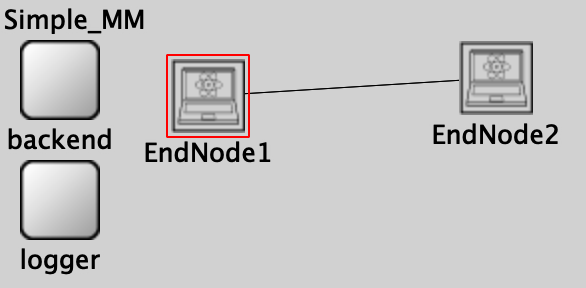
\includegraphics[width=.6\columnwidth]{images/topology_MM.png}}
  \caption{The figure of the network topology used in the experiment}
\end{figure}

\subsubsection{Result}

\begin{figure}[H]
  \centerline{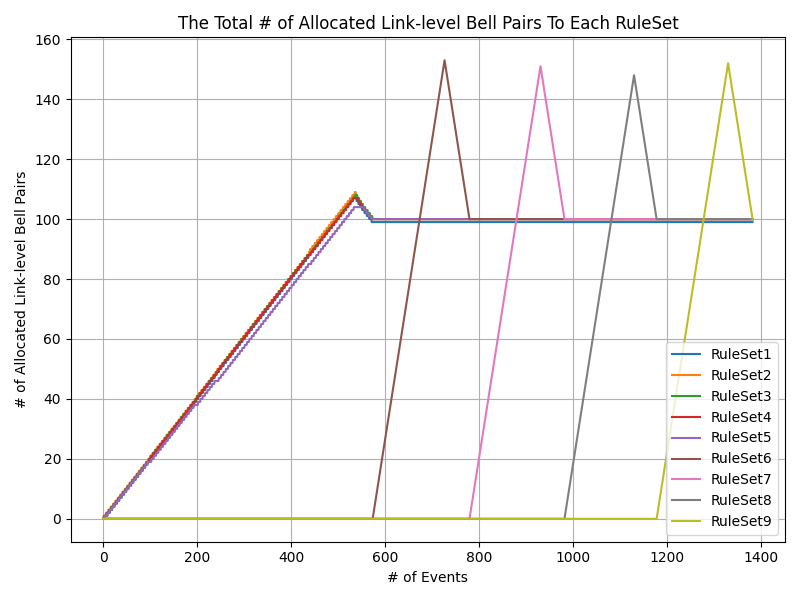
\includegraphics[width=.6\columnwidth]{images/result1.png}}
  \caption{The number of link-level Bell pairs allocated to each RuleSet}
  \label{fig:result1}
\end{figure}

Fig \ref{fig:result1} shows the number of link-level Bell pairs that are allocated to each RuleSet.
This figure shows that several RuleSets are already stored before the the generation of link-level Bell pairs is notified, and link-level Bell pairs are allocated to those RuleSet once the generation starts, which is a clear sign of multiplexing on a RuleSet-based quantum network.
It also shows that the number of allocated link-level Bell pairs declines.  This clearly indicates that link-level Bell pairs that are allocated but not consumed by each RuleSet were released after the relevant connection is torn down.

\newpage

\subsection{The Case When More Link-level Bell Pairs Are Required}

\subsubsection{Setting}
Table \ref{table:parameter-for-experiment2} is the table of parameters that are used in this experiment.

\begin{table}[ht]
  \begin{center}
    \begin{tabular}{|c|c|} 
      \hline
      Parameter & Value \\ \hline \cline{1-2}
      Total simulation time (s) &  20 \\ \cline{1-2}
      Waiting time for the initial notification of link generation (s) &  10 \\ \cline{1-2} 
      Interval for sending each ConnectionSetupRequest (s) &  2 \\ \cline{1-2} 
      Number of qubits in the buffer & 100  \\  \cline{1-2}
      Number of link-level Bell pairs required by each RuleSet &  200 \\ \cline{1-2}
      The type of RuleSet & Tomography \\  \hline  \cline{1-2}
    \end{tabular}
    \caption{A table of parameters in the experiment}
    \label{table:parameter-for-experiment2}
  \end{center}
\end{table}

\subsubsection{Result}

% 200 bell pairs, but 100 buffers
\begin{figure}[H]
  \centerline{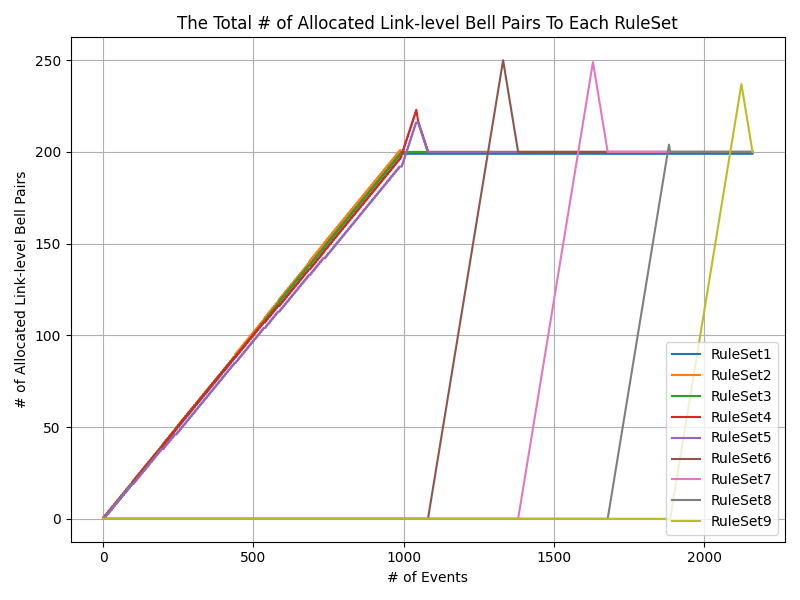
\includegraphics[width=.6\columnwidth]{images/result2.png}}
  \caption{The figure of the number of link-level Bell pairs allocated to each RuleSet}
  \label{fig:result2}
\end{figure}

Each RuleSet in this experiment requires twice as many link-level Bell pairs as how many Bell pairs generated in each round.
Fig \ref{fig:result2} shows that it takes more than one thousands events to finish multiplexing, which is more than twice as many events as how many it took in the previous experiment.


\newpage

\subsection{The Case When More Link-level Bell Pairs Are Generated}

\subsubsection{Setting}
Table \ref{table:parameter-for-experiment3} is the table of parameters that are used in this experiment.

\begin{table}[ht]
  \begin{center}
    \begin{tabular}{|c|c|} 
      \hline
      Parameter & Value \\ \hline \cline{1-2}
      Total simulation time (s) &  20 \\ \cline{1-2}
      Waiting time for the initial notification of link generation (s) &  10 \\ \cline{1-2} 
      Interval for sending each ConnectionSetupRequest (s) &  2 \\ \cline{1-2} 
      Number of qubits in the buffer & 200  \\  \cline{1-2}
      Number of link-level Bell pairs required by each RuleSet &  100 \\ \cline{1-2}
      The type of RuleSet & Tomography \\  \hline  \cline{1-2}
    \end{tabular}
    \caption{A table of parameters in the experiment}
    \label{table:parameter-for-experiment3}
  \end{center}
\end{table}

\subsubsection{Result}
% 100 bell pairs, but 200 buffers
\begin{figure}[H]
  \centerline{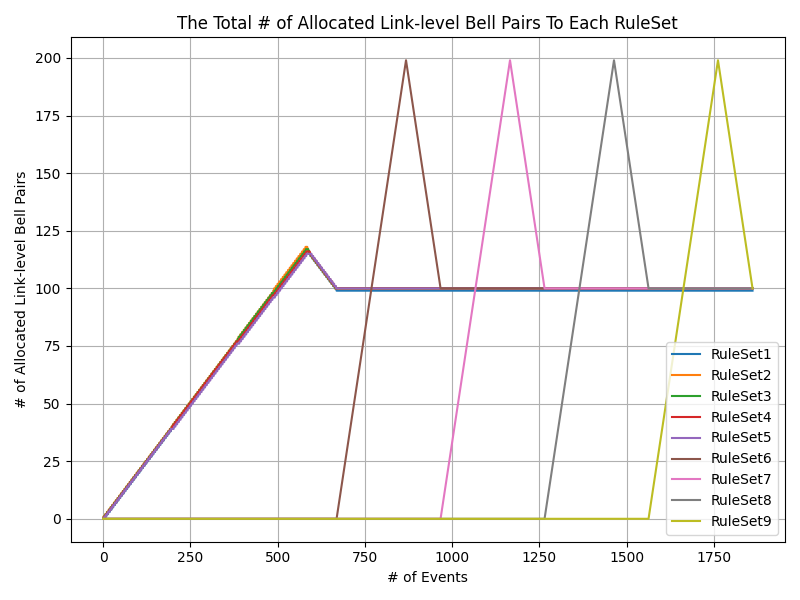
\includegraphics[width=.6\columnwidth]{images/result3.png}}
  \caption{The figure of the number of link-level Bell pairs allocated to each RuleSet}
  \label{fig:result3}
\end{figure}

The number of link-level Bell pairs generated in each round is twice as many as how many it is required by each RuleSet.
In the two previous experiments, one hundred link-level Bell pairs are generated in each round and more than one hundred link-level Bell pairs are allocated to a single RuleSet, which means that it takes more than one round of the generation of link-level Bell pairs until the execution of each RuleSet is terminated.
However, this experiment takes only one round of the generation of link-level Bell pairs until a single RuleSet is successfully executed.  This means that it is more time-efficient if the number of link-level Bell pairs generated in each round exceeds that of the total number of those required by a single RuleSet. 




%%% Local Variables:
%%% mode: japanese-latex
%%% TeX-master: "./thesis"
%%% End:
